\documentclass[tikz,border=5pt]{standalone}
\usepackage[T1]{fontenc}
\usepackage[utf8]{inputenc}
\usepackage[icelandic]{babel}
\usepackage{lmodern,amsmath,amssymb}
\usetikzlibrary{arrows.meta,calc,angles,quotes}
\definecolor{lotaBlue}{HTML}{073B63}
\definecolor{lotaGreen}{HTML}{19756D}
\definecolor{lotaCyan}{HTML}{408B9B}
\definecolor{lotaMagenta}{HTML}{A8588C}
\definecolor{ink}{HTML}{24342F}
\tikzset{every picture/.style={line width=.8pt,draw=lotaBlue,text=ink},>=Stealth}
\begin{document}
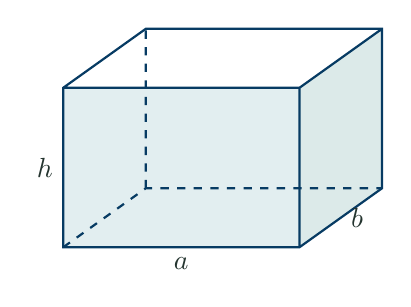
\begin{tikzpicture}[scale=.75]
\coordinate (A) at (0,0);\coordinate (B) at (4,0);\coordinate (C) at (5.4,1);\coordinate (D) at (1.4,1);
\coordinate (E) at (0,2.7);\coordinate (F) at (4,2.7);\coordinate (G) at (5.4,3.7);\coordinate (H) at (1.4,3.7);
\fill[lotaCyan!15] (A)--(B)--(F)--(E)--cycle;\fill[lotaGreen!15] (B)--(C)--(G)--(F)--cycle;
\draw (A)--(B)--(C)--(G)--(H)--(E)--cycle (E)--(F)--(G) (B)--(F);
\draw[dashed] (A)--(D)--(C) (D)--(H);
\node[below] at (2,0){$a$};\node[right] at (4.7,.5){$b$};\node[left] at (0,1.35){$h$};
\end{tikzpicture}

\begin{tikzpicture}[scale=.62]
\foreach \x/\y in {0/0,1.5/0,3/0,4.5/0,1.5/1.5,1.5/-1.5}{\draw[fill=lotaCyan!16] (\x,\y) rectangle ++(1.5,1.5);}
\node[above] at (2.25,3){$s=3{,}5$ cm};
\node[right,align=left] at (6.7,.8){Sex ferningar\\verða sex fletir.};
\end{tikzpicture}

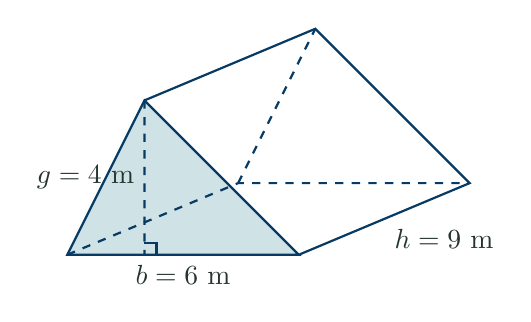
\begin{tikzpicture}[scale=.7]
\coordinate (A) at (0,0);\coordinate (B) at (4.2,0);\coordinate (C) at (1.4,2.8);
\fill[lotaCyan!25] (A)--(B)--(C)--cycle;
\draw (A)--(B)--(C)--cycle (B)--node[midway,below right]{$h=9$ m}(7.3,1.3)--(4.5,4.1)--(C);
\draw[dashed] (A)--(3.1,1.3)--(7.3,1.3) (3.1,1.3)--(4.5,4.1);
\draw[dashed] (C)--node[left]{$g=4$ m}(1.4,0);\draw (1.4,.22)--(1.62,.22)--(1.62,0);
\node[below] at (2.1,0){$b=6$ m};
\end{tikzpicture}

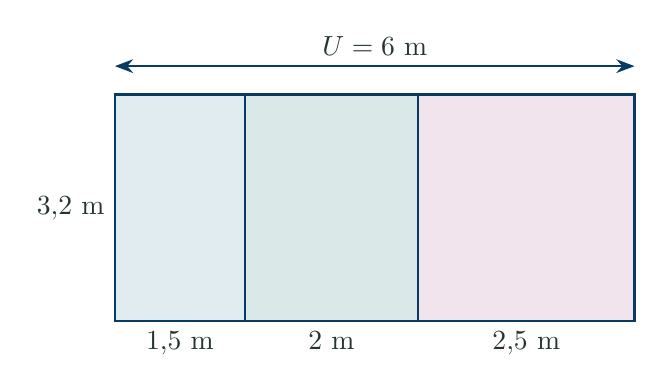
\begin{tikzpicture}[x=1.1cm,y=.9cm]
\draw[fill=lotaCyan!16] (0,0) rectangle (1.5,3.2);
\draw[fill=lotaGreen!16] (1.5,0) rectangle (3.5,3.2);
\draw[fill=lotaMagenta!16] (3.5,0) rectangle (6,3.2);
\node[below] at (.75,0){$1{,}5$ m};\node[below] at (2.5,0){$2$ m};\node[below] at (4.75,0){$2{,}5$ m};
\node[left] at (0,1.6){$3{,}2$ m};\draw[<->] (0,3.6)--node[above]{$U=6$ m}(6,3.6);
\end{tikzpicture}

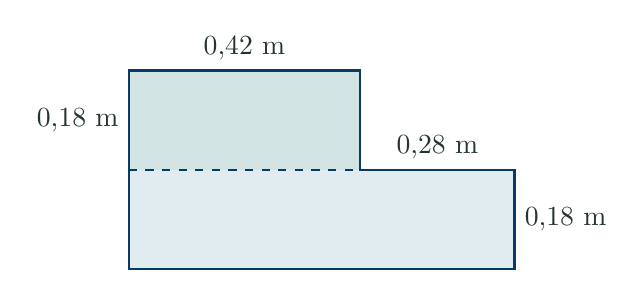
\begin{tikzpicture}[x=7cm,y=7cm]
\fill[lotaCyan!16] (0,0) rectangle (.7,.18);
\fill[lotaGreen!20] (0,.18) rectangle (.42,.36);
\draw (0,0)--(.7,0)--(.7,.18)--(.42,.18)--(.42,.36)--(0,.36)--cycle;
\draw[dashed] (0,.18)--(.42,.18);
\node[above] at (.21,.36){$0{,}42$ m};\node[above] at (.56,.18){$0{,}28$ m};
\node[right] at (.7,.09){$0{,}18$ m};\node[left] at (0,.27){$0{,}18$ m};
\end{tikzpicture}

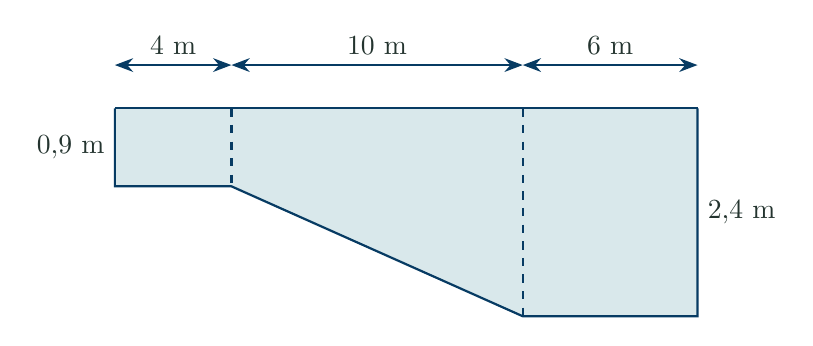
\begin{tikzpicture}[x=.37cm,y=1.1cm]
\fill[lotaCyan!20] (0,0)--(20,0)--(20,-2.4)--(14,-2.4)--(4,-.9)--(0,-.9)--cycle;
\draw[thick] (0,0)--(0,-.9)--(4,-.9)--(14,-2.4)--(20,-2.4)--(20,0);
\draw[lotaBlue] (0,0)--(20,0);
\draw[dashed] (4,0)--(4,-.9) (14,0)--(14,-2.4);
\draw[<->] (0,.5)--node[above]{4 m}(4,.5);
\draw[<->] (4,.5)--node[above]{10 m}(14,.5);
\draw[<->] (14,.5)--node[above]{6 m}(20,.5);
\node[left] at (0,-.45){$0{,}9$ m};\node[right] at (20,-1.2){$2{,}4$ m};
\end{tikzpicture}

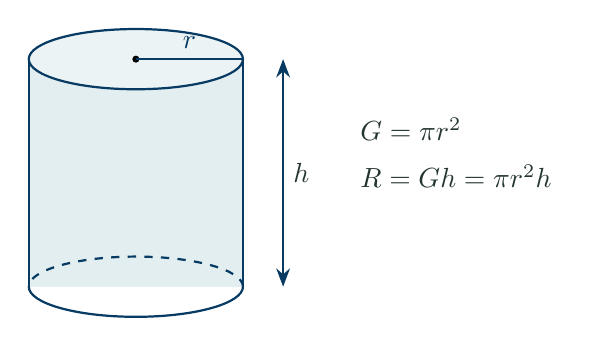
\begin{tikzpicture}[scale=.85]
\fill[lotaCyan!15] (-1.6,0) rectangle (1.6,3.4);
\draw (-1.6,0)--(-1.6,3.4) (1.6,0)--(1.6,3.4);
\draw[fill=lotaCyan!10] (0,3.4) ellipse (1.6 and .45);
\draw (1.6,0) arc[start angle=0,end angle=-180,x radius=1.6,y radius=.45];
\draw[dashed] (1.6,0) arc[start angle=0,end angle=180,x radius=1.6,y radius=.45];
\fill (0,3.4) circle(1.5pt);\draw[lotaBlue,thick] (0,3.4)--node[above]{$r$}(1.6,3.4);
\draw[<->] (2.2,0)--node[right]{$h$}(2.2,3.4);
\node[align=left,right] at (3.2,2){$G=\pi r^2$\\[5pt]$R=Gh=\pi r^2h$};
\end{tikzpicture}

\begin{tikzpicture}
\draw[fill=lotaCyan!18] (0,0) rectangle (6.2,2.1);
\draw[<->] (0,-.45)--node[below]{$U=2\pi r=\pi\text{\th}$}(6.2,-.45);
\draw[<->] (6.65,0)--node[right]{$h$}(6.65,2.1);
\node at (3.1,1.05){$M=2\pi rh$};
\end{tikzpicture}

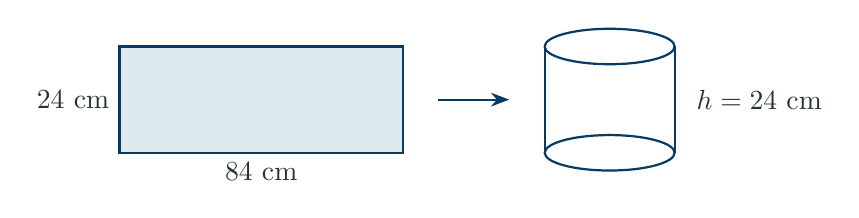
\begin{tikzpicture}[scale=.75]
\draw[fill=lotaCyan!18] (0,0) rectangle (4.8,1.8);
\node[below] at (2.4,0){84 cm};\node[left] at (0,.9){24 cm};
\draw[->,thick] (5.4,.9)--(6.6,.9);
\draw (7.2,0)--(7.2,1.8) (9.4,0)--(9.4,1.8);
\draw (8.3,1.8) ellipse (1.1 and .3);\draw (8.3,0) ellipse (1.1 and .3);
\node[right] at (9.6,.9){$h=24$ cm};
\end{tikzpicture}

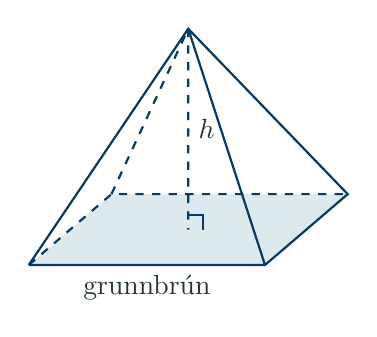
\begin{tikzpicture}[scale=.75]
\coordinate (A) at (0,0);\coordinate (B) at (4,0);\coordinate (C) at (5.4,1.2);\coordinate (D) at (1.4,1.2);\coordinate (T) at (2.7,4);
\fill[lotaCyan!18] (A)--(B)--(C)--(D)--cycle;
\draw (A)--(B)--(C)--(T)--(A) (B)--(T);
\draw[dashed] (A)--(D)--(C) (D)--(T) (T)--node[right]{$h$}(2.7,.6);
\draw (2.7,.85)--(2.95,.85)--(2.95,.6);\node[below] at (2,0){grunnbrún};
\end{tikzpicture}

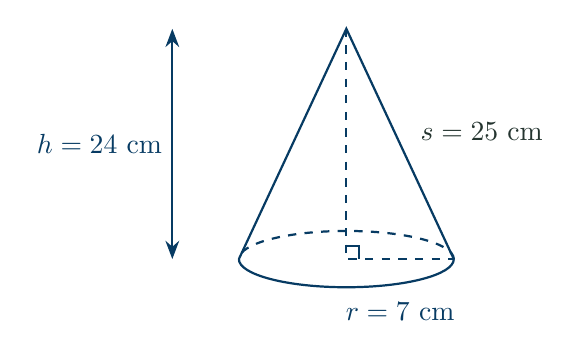
\begin{tikzpicture}[scale=.65]
\coordinate (T) at (0,4.5);\coordinate (O) at (0,0);\coordinate (P) at (2.1,0);
\draw (-2.1,0)--(T)--(P);
\draw (2.1,0) arc[start angle=0,end angle=-180,x radius=2.1,y radius=.55];
\draw[dashed] (2.1,0) arc[start angle=0,end angle=180,x radius=2.1,y radius=.55];
\draw[dashed,lotaBlue] (T)--(O)--node[below=12pt]{$r=7$ cm}(P);
\draw[<->,lotaBlue] (-3.4,0)--node[left]{$h=24$ cm}(-3.4,4.5);
\draw (0,.25)--(.25,.25)--(.25,0);
\node[right] at (1.25,2.5){$s=25$ cm};
\end{tikzpicture}

\begin{tikzpicture}[scale=.8]
\draw (-1.5,1.4)--(-1.5,4.2) (1.5,1.4)--(1.5,4.2);
\draw (0,4.2) ellipse(1.5 and .4);
\draw[dashed] (0,1.4) ellipse(1.5 and .4);
\draw (-1.5,1.4)--(0,0)--(1.5,1.4);
\draw[<->] (2,1.4)--node[right]{$1{,}4$ m}(2,4.2);
\draw[<->] (2,0)--node[right]{$0{,}5$ m}(2,1.4);
\draw[<->] (-1.5,4.9)--node[above]{$\text{\th}=1{,}2$ m}(1.5,4.9);
\end{tikzpicture}

\begin{tikzpicture}[scale=.85]
\draw[fill=lotaCyan!10] (0,0) circle(1.65);
\draw (1.65,0) arc[start angle=0,end angle=-180,x radius=1.65,y radius=.43];
\draw[dashed] (1.65,0) arc[start angle=0,end angle=180,x radius=1.65,y radius=.43];
\fill (0,0) circle(1.5pt);\draw[lotaBlue,thick] (0,0)--node[above]{$r$}(1.65,0);
\node[right,align=left] at (2.6,.3){Rúmmál: $\displaystyle R=\frac43\pi r^3$\\[12pt]Yfirborð: $Y=4\pi r^2$};
\end{tikzpicture}

\begin{tikzpicture}[scale=.65]
\draw[fill=lotaCyan!15] (-2.5,0) arc[start angle=180,end angle=0,radius=2.5]--cycle;
\draw (1.5,1.6) arc[start angle=180,end angle=0,radius=2.5];
\draw (-2.5,0)--(1.5,1.6) (2.5,0)--(6.5,1.6) (0,2.5)--(4,4.1);
\draw[dashed] (1.5,1.6)--(6.5,1.6);
\node[below] at (0,0){$\text{\th}=5$ m};\node[below right] at (4.5,.8){$L=12$ m};
\end{tikzpicture}

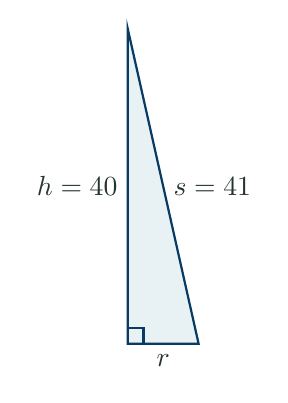
\begin{tikzpicture}[x=.10cm,y=.10cm]
\draw[fill=lotaCyan!12] (0,0)--(9,0)--(0,40)--cycle;
\draw (0,2)--(2,2)--(2,0);
\node[left] at (0,20){$h=40$};\node[below] at (4.5,0){$r$};\node[right] at (4.5,20){$s=41$};
\end{tikzpicture}

\begin{tikzpicture}[x=.15cm,y=.15cm]
\draw[fill=lotaCyan!12] (0,0) rectangle (7,24);
\draw[lotaBlue,thick] (0,24)--(7,0);
\node[right,lotaBlue] at (10,12){$25$};\draw[->,lotaBlue] (10,12)--(3.5,12);
\node[left] at (0,12){$24$};\node[below] at (3.5,0){$\text{\th}$};
\draw (0,1.5)--(1.5,1.5)--(1.5,0);
\end{tikzpicture}

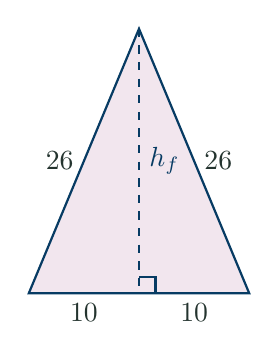
\begin{tikzpicture}[x=.14cm,y=.14cm]
\draw[fill=lotaMagenta!15] (-10,0)--(10,0)--(0,24)--cycle;
\draw[dashed,lotaBlue] (0,24)--node[right]{$h_f$}(0,0);
\draw (0,1.5)--(1.5,1.5)--(1.5,0);
\node[below] at (-5,0){10};\node[below] at (5,0){10};
\node[right] at (5,12){26};\node[left] at (-5,12){26};
\end{tikzpicture}

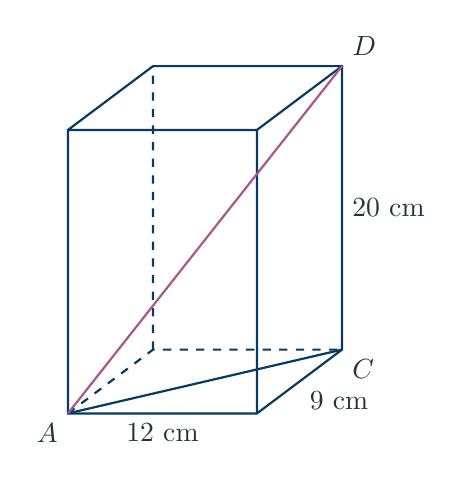
\begin{tikzpicture}[scale=.6]
\coordinate(A)at(0,0);\coordinate(B)at(4,0);\coordinate(C)at(5.8,1.35);\coordinate(E)at(1.8,1.35);
\coordinate(F)at(0,6);\coordinate(G)at(4,6);\coordinate(D)at(5.8,7.35);\coordinate(H)at(1.8,7.35);
\draw(A)--(B)--(C)--(D)--(H)--(F)--cycle (F)--(G)--(D) (B)--(G);
\draw[dashed](A)--(E)--(C) (E)--(H);
\draw[lotaBlue,thick](A)--(C);\draw[lotaMagenta,thick](A)--(D);
\node[below left]at(A){$A$};\node[below right]at(C){$C$};\node[above right]at(D){$D$};
\node[below]at(2,0){12 cm};\node[below right]at(4.9,.675){9 cm};\node[right]at(5.8,4.35){20 cm};
\end{tikzpicture}

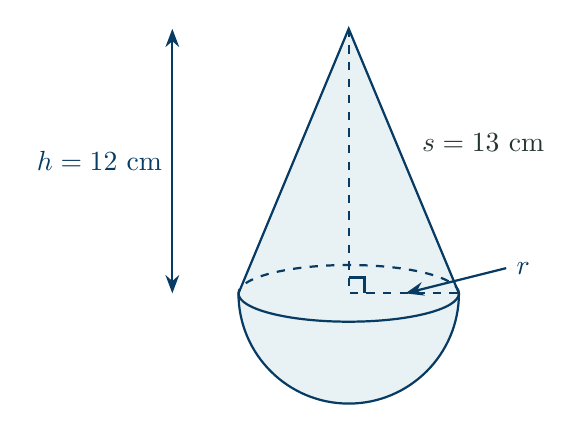
\begin{tikzpicture}[scale=.8]
\draw[fill=lotaCyan!12] (-1.75,0)--(0,4.2)--(1.75,0) arc[start angle=0,end angle=-180,radius=1.75]--cycle;
\draw (1.75,0) arc[start angle=0,end angle=-180,x radius=1.75,y radius=.45];
\draw[dashed] (1.75,0) arc[start angle=0,end angle=180,x radius=1.75,y radius=.45];
\draw[dashed,lotaBlue] (0,4.2)--(0,0)--(1.75,0);
\draw[<->,lotaBlue] (-2.8,0)--node[left]{$h=12$ cm}(-2.8,4.2);
\node[right,lotaBlue] at (2.5,.4){$r$};\draw[->,lotaBlue] (2.5,.4)--(.9,0);
\draw (0,.25)--(.25,.25)--(.25,0);\node[right] at (1,2.4){$s=13$ cm};
\end{tikzpicture}\end{document}